\documentclass[12pt]{article}
\usepackage[pdftex]{graphicx}

\newcommand{\kg}{\mathrm{kg}}
\newcommand{\m}{\mathrm{m}}
\newcommand{\cm}{\mathrm{cm}}
\newcommand{\km}{\mathrm{km}}
\newcommand{\s}{\mathrm{s}}
\renewcommand{\min}{\mathrm{min}}
\newcommand{\ms}{\mathrm{ms}}
\newcommand{\N}{\mathrm{N}}
\newcommand{\vs}{\emph{vs}}
\newcommand{\abs}[1]{\left|{#1}\right|}

\newcounter{problem}
\stepcounter{problem}
\newcounter{answer}[problem]
\newenvironment{problem}{\noindent\begin{minipage}{\textwidth}\sloppy\sloppypar\raggedright\textbf{\theproblem.}\refstepcounter{problem}\stepcounter{answer}---}{\end{minipage}\vspace{2ex}}
\newcommand{\source}[1]{[{#1}]}
\newenvironment{answers}{\\}{}
\newcommand{\answer}[1]{\mbox{\textbf{\Alph{answer}:}\refstepcounter{answer}~{#1}\hspace{3ex}}}
\begin{document}

\section*{NYU General Physics 1---Term Exam 1}

\begin{problem}
  \source{from lecture 2011-09-03} How long does it take a heavy
  bucket to fall three stories?
  \begin{answers}
    \answer{about a microsecond}
    \answer{about a millisecond}
    \answer{about a tenth of a second}
    \answer{about a second}
  \end{answers}
\end{problem}

%% \begin{problem}
%%   \source{from lecture 2011-09-05} What is the mass of a pint of beer?
%%   \begin{answers}
%%     \answer{$0.05\,\kg$}
%%     \answer{$0.5\,\kg$}
%%     \answer{$5\,\kg$}
%%   \end{answers}
%% \end{problem}

\begin{problem}
  \source{from lecture 2011-09-05} What is the radius of the Earth, roughly?
  \begin{answers}
    \answer{$6,000\,\m$}
    \answer{$200\,\km$}
    \answer{$6,000\,\km$}
    \answer{$200,000\,\km$}
  \end{answers}
\end{problem}

\begin{problem}
  \source{from lecture 2011-09-10} We analyzed a stone thrown from a
  cliff, ignoring air resistance.  The velocity changes continuously
  with time.  What aspect of the velocity \emph{stays the same} throughout
  the trajectory?
  \begin{answers}
    \answer{the magnitude}
    \answer{the direction}
    \answer{the vertical component (or projection)}
    \answer{the horizontal component (or projection)}
    \answer{none of these}
  \end{answers}
\end{problem}

\begin{problem}
  \source{from lecture 2011-09-12} You are driving in the positive-$x$
  direction.  You hit the brakes.  As you are braking, what is the
  ``kinematic state'' of the vehicle?
  \begin{answers}
    \answer{$v_x > 0$, $a_x > 0$}
    \answer{$v_x > 0$, $a_x < 0$}
    \answer{$v_x < 0$, $a_x > 0$}
    \answer{$v_x < 0$, $a_x < 0$}
  \end{answers}
\end{problem}

\begin{problem}
  \source{from lecture 2011-09-17} What does ``frictionless'' mean?
  \begin{answers}
    \answer{no contact force parallel to the surface}
    \answer{no contact force perpendicular to the surface}
    \answer{no contact force from the surface}
    \answer{perfectly smooth}
    \answer{perfectly rigid}
  \end{answers}
\end{problem}

\begin{problem}
  \source{from lecture 2011-09-17} For the problem of the block of
  mass $m$ on the frictionless, inclined plane (inclined at an angle
  $\theta$ to the horizontal), what is a possibly reasonable formula
  for the magnitude of the normal force?
  \begin{answers}
    \answer{$\abs{\vec{N}} = m\,\abs{\vec{g}}\,\cos\theta$}
    \answer{$\abs{\vec{N}} = m\,\abs{\vec{g}}\,\sin\theta$}
    \answer{$\abs{\vec{N}} = \frac{m\,\abs{\vec{g}}}{\cos\theta}$}
    \answer{$\abs{\vec{N}} = \frac{m\,\abs{\vec{g}}}{\sin\theta}$}
    \answer{none of those is reasonable}
  \end{answers}
\end{problem}

\begin{problem}
  \source{from lecture 2011-09-17}  For the problem of the block of
  mass $m$ on the frictionless, inclined plane (inclined at an angle
  $\theta$ to the horizontal), what simplifying assumption did we \emph{not need to make}?
  \begin{answers}
    \answer{The plane is frictionless.}
    \answer{The block will accelerate parallel to the plane.}
    \answer{Air resistance is negligible (can be ignored).}
    \answer{The block was released from rest (zero velocity).}
  \end{answers}
\end{problem}

\begin{problem}
  \source{from lecture 2011-09-19} Two masses $m_1$ and $m_2$ hang by
  a light, inextensible string over a pulley.  What is a
  \emph{possible and reasonable} formula for the magnitude of the
  acceleration of mass $m_1$?
  \begin{answers}
    \answer{$\displaystyle\abs{\vec{a}} = \abs{\frac{(m_1 - m_2)}{(m_1 + m_2)}\,\vec{g}}$}
    \answer{$\displaystyle\abs{\vec{a}} = \abs{\frac{(m_1 + m_2)}{(m_1 - m_2)}\,\vec{g}}$}
    \answer{$\displaystyle\abs{\vec{a}} = \abs{(m_1 - m_2)\,\vec{g}}$}
    \answer{$\displaystyle\abs{\vec{a}} = \abs{(m_1 + m_2)\,\vec{g}}$}
    \answer{these are all unreasonable}
  \end{answers}
\end{problem}

\begin{problem}
  \source{from problem set 1, problem 1} What, roughly, is the mass of
  a single dollar bill?
  \begin{answers}
    \answer{$0.00003\,\kg$}
    \answer{$0.001\,\kg$}
    \answer{$0.03\,\kg$}
    \answer{$1\,\kg$}
    \answer{$3\,\kg$}
  \end{answers}
\end{problem}

\begin{problem}
  \source{from problem set 1, problem 2} You computed a ``power'' for
  air resistance, involving speed, density, and area.  If one car is
  going twice as fast as another car, but the two cars are identical
  in every other respect (same size and shape and mass), how much
  larger is this air-resistance power for the faster-moving car?
  \begin{answers}
    \answer{not larger; in fact exactly the same}
    \answer{larger by a factor of $2$}
    \answer{larger by a factor of $4$}
    \answer{larger by a factor of $8$}
    \answer{none of the above}
  \end{answers}
\end{problem}

\begin{problem}
  \source{from problem set 1, problem 3} You computed an approximate
  settling velocity for particles in a centrifuge (and you used the
  units of dynamic viscosity, $\kg\,\m^{-1}\,\s^{-1}$). If you hold
  density and gravitational acceleration fixed, how does the settling
  velocity depend on particle size?
  \begin{answers}
    \answer{larger velocity for larger particles}
    \answer{velocity doesn't depend on particle size}
    \answer{smaller velocity for larger particles}
  \end{answers}
\end{problem}

\begin{problem}
  \source{from problem set 2, problem 1} What is a reasonable value
  for the mean acceleration of a dragster in a drag race, very
  roughly?
  \begin{answers}
    \answer{$0.03\,\m\,\s^{-2}$}
    \answer{$1\,\m\,\s^{-2}$}
    \answer{$30\,\m\,\s^{-2}$}
    \answer{$1000\,\m\,\s^{-2}$}
  \end{answers}
\end{problem}

\begin{problem}
  \source{from problem set 2, problem 2} You drew a graph of the
  position $y$ (height) as a function of time for a rock that is
  thrown precisely upwards at $3~\mathrm{m\,s^{-1}}$ at time $t=0$.
  What is the maximum height to which the rock rose, above the
  starting point?  Use $\abs{\vec{g}}=10\,\m\,\s^{-2}$ to answer this.
  \begin{answers}
    \answer{$0.45\,\m$}
    \answer{$0.9\,\m$}
    \answer{$2\,\m$}
    \answer{$3\,\m$}
    \answer{$30\,\m$}
  \end{answers}
\end{problem}

\begin{problem}
  \source{from problem set 2, problem 2} You drew a graph of the
  acceleration $a_y$ (vertical acceleration) as a function of time for
  a rock that is thrown upwards.  What happens to the acceleration
  \vs\ time graph at the exact moment that the rock gets to maximum
  height?
  \begin{answers}
    \answer{nothing special at all}
    \answer{the acceleration is undefined}
    \answer{the acceleration is zero}
    \answer{the acceleration changes sign}
    \answer{the slope of the $a_y$ \vs\ $t$ graph changes sign}
  \end{answers}
\end{problem}

\begin{problem}
  \source{from problem set 2, problem 3} You integrated this velocity
  curve:\\ 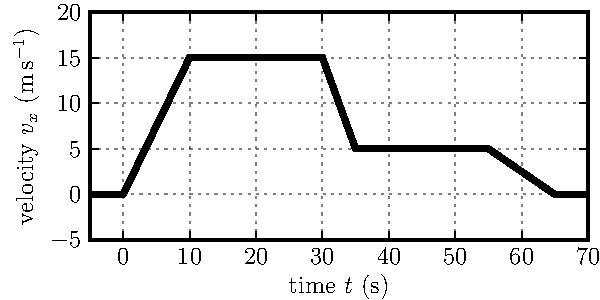
\includegraphics{../py/vx_vs_t.pdf}\\ What is the position
  $x$ at $t=35\,\s$?  Assume that $x=0$ at $t=0$.
  \begin{answers}
    \answer{$5\,\m$}
    \answer{$175\,\m$}
    \answer{$412.5\,\m$}
    \answer{$425\,\m$}
    \answer{$525\,\m$}
  \end{answers}
\end{problem}

\begin{problem}
  \source{from problem set 3, problem 1} If the acceleration due to
  gravity $g$ were \emph{doubled} (to, say, $20\,\m\,\s^{-2}$), but
  everything \emph{else} about the Earth (radius especially) remained
  the same, what (roughly) would be the orbital period of the Space
  Shuttle?
  \begin{answers}
    \answer{$45\,\min$}
    \answer{$66\,\min$}
    \answer{$90\,\min$}
    \answer{$126\,\min$}
    \answer{$180\,\min$}
  \end{answers}
\end{problem}

\begin{problem}
  \source{from problem set 3, problem 2} You solved for the tension
  $T$ in this
  problem:\\ 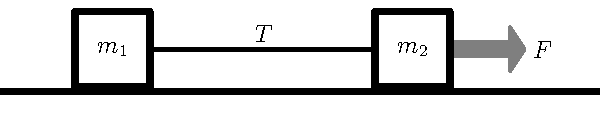
\includegraphics{../py/stringblocks.pdf}\\ Now imagine
  that the mass $m_2$ is much, much smaller than the mass $m_1$.  What
  is the tension $T$ in the (light, inextensible) string in this
  special case?
  \begin{answers}
    \answer{very close to zero}
    \answer{very close to $F$}
    \answer{very close to $\frac{F}{m_1}$}
    \answer{very close to $\frac{F}{m_2}$}
    \answer{not close to any of these answers}
  \end{answers}
\end{problem}

\begin{problem}
  \source{from problem set 3, problem 3} A block of mass $m=7\,\kg$
  lies on a horizontal table.  It is stationary relative to the table,
  which is accelerating upwards (in, say, an elevator).  You found the
  normal force $N$ between the table and the block when the table is
  accelerating upwards at $0.9\,\m\,\s^{-2}$.  If you reduced this
  upwards acceleration to $0.3\,\m\,\s^{-2}$, what would happen to
  the magnitude of the normal force?
  \begin{answers}
    \answer{it would get smaller by a factor of three}
    \answer{it would get smaller by about five percent}
    \answer{it would stay the same}
    \answer{it would get larger by about five percent}
    \answer{it would get larger by a factor of three}
  \end{answers}
\end{problem}

\begin{problem}
  \source{from \textit{Motion 1} lab} If your plot of position
  \vs\ time looks like a straight line, what does that mean, in
  general?
  \begin{answers}
    \answer{the object isn't moving}
    \answer{the object is moving in the positive direction}
    \answer{the object is moving at constant speed}
    \answer{the object is accelerating at constant acceleration}
    \answer{none of the above}
  \end{answers}
\end{problem}

\begin{problem}
  \source{from \textit{Motion 2} lab} When you measure
  accelerations of gliders of different masses on a track at a
  constant angle $\theta$, what is the expectation?
  \begin{answers}
    \answer{more massive things should have substantially higher accelerations}
    \answer{everything should accelerate at the pretty much same rate}
    \answer{more massive things should have substantially lower accelerations}
  \end{answers}
\end{problem}

\end{document}
